\title[Causality]{Causality: Lecture 9}
\author[Joris Mooij]{\\[5mm]\large Joris Mooij \& Patrick Forr\'e\\
\url{j.m.mooij@uva.nl}, \url{p.d.forre@uva.nl}}
\institute[UvA]{University of Amsterdam}
\date[2025-04-04]{\normalsize April 4th, 2025}
\maketitle


\part{Structural Causal Models (with Inputs)}
\frame{\partpage}

\begin{frame}[t]{Beyond Causal Bayesian Networks}
  Consider:\\

  \bigskip
  \begin{tabular}{ll}
    $v_1$ & Annual amount of sunlight absorbed at the North pole \\
    $v_2$ & Average annual temperature in the area \\
    $v_3$ & Fraction of sea covered by ice in the area \\
  \end{tabular}

  \bigskip
  What CBN could we use to model this?

  \bigskip
  \bigskip
  \bigskip
  \centerline{\begin{tikzpicture} 
  \begin{scope}
    \node[ndout] (v1) at (0,2.8) {$v_1$};
    \node[ndout] (v2) at (2,2.8) {$v_2$};
    \node[ndout] (v3) at (1,1.2) {$v_3$};
    \uncover<2- |handout:0>{
%    \draw[arout, out=30, in=150] (v1) to (v2);
%    \draw[arout, out=-90, in=30] (v2) to (v3);
%    \draw[arout, out=150, in=-90] (v3) to (v1);
    \draw[arout] (v1) to (v2);
    \draw[arout] (v2) to (v3);
    \draw[arout] (v3) to (v1);
  }
  \end{scope}
  \end{tikzpicture}}
  \uncover<2- |handout:0>{Contradiction!}
\end{frame}

\begin{frame}[t]{Merging variables may introduce cycles}
  Causal cycles can also be introduced by using a representation that is too coarse:

  \bigskip
  \bigskip
  \centerline{\begin{tikzpicture}[scale=1, transform shape]
  \begin{scope}
    \node[ndout] (v1) at (0,0) {$v_1$};
    \node[ndout] (v2) at (0,-2) {$v_2$};
    \node[ndout] (v3) at (1.5,0) {$v_3$};
    \node[ndout] (v4) at (1.5,-2) {$v_4$};
    \draw[arout] (v1) to (v2);
    \draw[arout] (v4) to (v3);
  \end{scope}
  \begin{scope}[xshift=6cm]
    \node[ndout] (v13) at (0,0) {$v_{13}$};
    \node[ndout] (v24) at (0,-2) {$v_{24}$};
%    \node[ndout] (v3) at (1,0) {$v_3$};
%    \node[ndout] (v4) at (1,-2) {$v_4$};
    \uncover<2- |handout:0>{%
      \draw[arout,bend left] (v13) to (v24);
      \draw[arout,bend left] (v24) to (v13);
    }
  \end{scope}
  \end{tikzpicture}}

  \bigskip
  \bigskip
  Left: four variables $X_1, X_2, X_3, X_4$\\
  Right: two merged variables $(X_1,X_3), (X_2,X_4)$.

  \bigskip
  \uncover<2- |handout:0>{Contradiction!}
\end{frame}

\begin{frame}{Context-dependent causal relations}
Different causal models corresponding to modeling the current through a resistance using Ohm's law $V = IR$:

\bigskip
\centerline{\begin{tikzpicture}[scale=0.9, transform shape]
  \begin{scope}[xshift=0cm]
    \node[ndout] (V) at (0,0) {$V$};
    \node[ndout] (I) at (2,0) {$I$};
    \node[ndint] (R) at (1,-1.5) {$R$};
    \uncover<2-|handout:0>{%
      \draw[arout] (V) to (I);
      \draw[arint] (R) to (I);
    }
  \end{scope}
  \begin{scope}[xshift=5cm]
    \node[ndout] (V) at (0,0) {$V$};
    \node[ndout] (I) at (2,0) {$I$};
    \node[ndint] (R) at (1,-1.5) {$R$};
    \uncover<2-|handout:0>{%
      \draw[arout] (I) to (V);
      \draw[arint] (R) to (V);
    }
  \end{scope}
  \begin{scope}[xshift=10cm]
    \node[ndout] (C) at (1,1.5) {$C$};
    \node[ndout] (V) at (0,0) {$V$};
    \node[ndout] (I) at (2,0) {$I$};
    \node[ndint] (R) at (1,-1.5) {$R$};
    \uncover<3-|handout:0>{%
      \draw[arout] (C) to (V);
      \draw[arout] (C) to (I);
      \draw[arout,bend left] (I) to (V);
      \draw[arout,bend left] (V) to (I);
      \draw[arint] (R) to (I);
      \draw[arint] (R) to (V);
    }
  \end{scope}
\end{tikzpicture}}

\bigskip
Left: Resistance connected to voltage source.\\
Center: Resistance connected to current source.\\
Right: Flip a coin; if `heads' connect resistance to voltage source, if `tails' connect resistance to current source. \uncover<3- |handout:0>{Contradiction!}

\bigskip
Such context-specific causality is often encountered in complex systems in chemistry, biology, economy, and engineering.
\end{frame}

\begin{frame}{Structural Causal Models (with Inputs)}
  Additional features of SCMs over L-CBNs:
  \begin{itemize}
    \item SCMs can deal with cycles;
    \item SCMs support graphical approaches to counterfactual reasoning.
  \end{itemize}
  We add:
  \begin{itemize}
    \item input variables,
  \end{itemize}
  giving \emph{iSCMs} = `\emph{SCM}s with \emph{i}nputs' (which extend L-CBNs).

  \bigskip
  A (brief) history of iSCMs:
  \begin{itemize}
    \item path analysis by geneticist Sewall Wright \cite{Wri21}
    \item Structural Equation Models (SEMs) in econometrics \cite{Wright1928,Haa43,StrotzWold1960} and social sciences \cite{Bollen1989}
    \item introduced into AI / ML by Judea Pearl \cite{Pearl09} and others
    \item measure-theoretic formulation \cite{BFPM21}
    \item extension to input nodes (these lecture notes).
  \end{itemize}
\end{frame}

\begin{frame}{iSCMs: Ingredients}
\begin{itemize}
  \item an iSCM is specified in terms of \emph{deterministic} functions and \emph{distributions} (rather than in terms of Markov kernels).
  \item An iSCM describes `modular' \emph{causal mechanisms} that fully determine an effect as a function of its direct causes.
  \item To prevent infinite regress, not all variables come with a causal mechanism:
    the \emph{endogenous} ones do, the \emph{exogenous} ones don't.
  \item We distinguish two types of exogenous variables:
    \begin{itemize}
      \item \emph{exogenous random variables} for which both their range and probability distribution is specified, and
      \item \emph{exogenous input variables} (only in iSCMs!) for which only their range is specified.
    \end{itemize}
\end{itemize}

Hence, we consider the following variable types:

\medskip
\centerline{\begin{tabular}{l|ll|ll}
  variable type    & SCM & iSCM & observable? & intervenable? \\
  \hline
  endogenous       & $+$   & $+$    & $+$          & $+$ \\
  exogenous random & $+$   & $+$    & $-$          & $-$ \\
  exogenous input  & $-$   & $+$    & $+$          & $+$ (intervened) \\
\end{tabular}}
\end{frame}

\begin{frame}{iSCMs: Definition}
  \begin{Def}[\ref{def:iscm}]
    A \emph{Structural Causal Model with Inputs (iSCM)} $M$ is a tuple $\lt \Sin, \Send, \Srnd, \CX, P, f \rt$ 
  where
  \begin{itemize}
    \item the \emph{exogenous input variables}, the \emph{endogenous variables} and the \emph{exogenous random variables} are indexed by disjoint (finite) index sets $\Sin, \Send, \Srnd$, respectively;
    \item the \emph{domain} $\CX = \prod_{i\in \Sin \cup \Send \cup \Srnd} \C{X}_i$ is a product of standard measurable spaces $\C{X}_i$;
    \item the \emph{exogenous distribution} $P$ is a probability distribution on $\CXW$ that factorizes as a product $P = \bigotimes_{w\in\Srnd} P_w$ of probability distributions $P_w \in \C{P}(\C{X}_w)$, one for each exogenous space $\C{X}_w$;
    \item the \emph{causal mechanisms} are specified by the measurable function $f : \CX \to \CXV$.
  \end{itemize}
\end{Def}
If $f$ and $P$ depend in a measurable way on \emph{exogenous parameters} $\theta\in\Theta$, 
we write $M^{\theta} = \lt \Sin, \Send, \Srnd, \CX, P^{\theta}, f^{\theta} \rt$.
\end{frame}

\begin{frame}{Remarks}
  An iSCM embodies the following modeling assumptions:
  \begin{enumerate}
    \item Exogenous variables (input, random, and parameters) are \emph{not caused by} the endogenous variables.
    \item Exogenous variables are \emph{variation independent}.
    \item Exogenous random variables are \emph{probabilistically independent}, and their distribution is \emph{independent} of the values of the exogenous input variables
      (but may depend on the exogenous parameters).
    \item Exogenous parameters describe \emph{population} properties, while exogenous random and input variables describe \emph{individual} quantities.
      That is, if we model $N$ units, they all share the same value of $\theta$.
  \end{enumerate}

  \bigskip
  Our definition of iSCMs is unconventional, as:
  \begin{enumerate}
    \item We allow for exogenous input variables (but for $J=\emptyset$ reduce to SCMs);
%    \item Often, endogenous variables are considered observed and exogenous random variables latent, but we make no such restriction.
    \item We allow for cyclic causal dependences between the endogenous variables.
  \end{enumerate}
\end{frame}

\begin{frame}{Potential Outcomes and Structural Equations}
\begin{Def}[\ref{def:scm_solutions_for_inputs}]
  Let $M = \lt \Sin, \Send, \Srnd, \CX, P, f \rt$ be an iSCM and $\xJ \in \CXJ$ an input value.
  A random variable $X_{V \cup W}^{\doit(\xJ)}$ with codomain $\CXV \times \CXW$ is called
  a \emph{potential outcome of $M$ for input $\xJ$} 
  if the following two conditions hold:
    \begin{enumerate}
      \item its $\Srnd$-component has the exogenous distribution specified by $M$: 
        $$\XW^{\doit(\xJ)} \sim P,$$
      \item it satisfies the \emph{structural equations entailed by $M$ for input $\xJ$}:
        \begin{equation*}
          \XV^{\doit(\xJ)} = f\big(\xJ, \XV^{\doit(\xJ)}, \XW^{\doit(\xJ)}\big) \text{ a.s.}.
        \end{equation*}
    \end{enumerate}
  In case $J = \emptyset$ we also write $X_{V \cup W} := X_{V \cup W}^{\doit(\asterisk)}$ and refer to it simply as an \emph{outcome of $M$}.
\end{Def}
A common way to write potential outcomes is as $X_{V\cup W}(\xJ)$.
\end{frame}

\begin{frame}[t]{Example 1}
Potential outcomes may not exist, or may not be unique.
\begin{Eg}
Consider an iSCM with structural equations
$$\begin{cases}
  X_1 = \alpha X_2 & \\
  X_2 = \beta X_1 + X_3. &
\end{cases}$$
with $X_3$ an exogenous input. What are its potential outcomes?

\bigskip
\uncover<2-|handout:0>{Answer:
  \begin{itemize}
    \item $\alpha \beta = 1$, $x_3=0$: $(X_1^{\doit(x_3=0)},X_2^{\doit(x_3=0)}) = (\alpha x,x)$ for any $x\in\RN$.\\
    Note: not unique; any mixture of these is also a potential outcome.
  \item $\alpha \beta = 1$, $x_3\ne 0$: no potential outcomes defined!
  \item $\alpha \beta \ne 1$: unique potential outcomes $(X_1^{\doit(x_3)},X_2^{\doit(x_3)}) = (\frac{\alpha x_3}{1 - \alpha\beta},\frac{x_3}{1 - \alpha\beta})$.
  \end{itemize}
}
\end{Eg}
\end{frame}

\begin{frame}{Example 2}
  \begin{Eg}[Linear regression model with fixed design for effect given cause, population level]
  $$Y = \alpha X + \beta + \epsilon$$ 
    $Y \in \RN$: effect; \quad $X \in \RN$: cause; \quad $\epsilon \sim \C{N}(0,\sigma^2)$: noise; \quad $\alpha,\beta \in \RN,\sigma^2 \in (0,\infty)$: parameters.

    \medskip
  This can be understood as the specification of an iSCM
    \begin{equation*}\begin{split}
      M^{(\alpha,\beta,\sigma^2)} 
      &= \lt \Sin = \{X\}, \Send = \{Y\}, \Srnd = \{\epsilon\}, \CX = \RN^3, \right. \\
        & \quad \left. P^{\sigma^2}(X_\epsilon) = \C{N}(0,\sigma^2), f^{\alpha,\beta} : \RN^3 \to \RN : (x,y,\epsilon) \mapsto \alpha x + \beta + \epsilon \rt
    \end{split}\end{equation*} 
  If $\epsilon \sim \C{N}(0,\sigma^2)$, then $(Y^{\doit(x)},\epsilon^{\doit(x)}) := (\alpha x + \beta + \epsilon, \epsilon)$ is
    a potential outcome of $M^{(\alpha,\beta,\sigma^2)}$. 
  %If $\epsilon$ is latent (which is usually the case), we just refer to $Y^{\doit(x)}$ as the potential outcome.
\end{Eg}
\end{frame}

\begin{frame}{Example 3}
\begin{Eg}[Now at the individual level]
  Expanding the template to a population of $N$ independent units:
  \begin{itemize}
    \item Exogenous input variable $J = \{X_1,\dots,X_N\}$;
    \item Exogenous random variable indices $W = \{\epsilon_1,\dots,\epsilon_N\}$;
    \item Endogenous variable indices $V = \{Y_1,\dots,Y_N\}$;
    \item Joint state space $\CX = \prod_{i=1}^N \CX_i = \prod_{i=1}^N (\RN \times \RN \times \RN) = \RN^{3N}$;
    \item Parameters $(\alpha,\beta,\sigma^2) \in \RN^2 \times (0,\infty)$;
    \item Exogenous distribution $P^\sigma(X_W) = \bigotimes_{i=1}^N P^\sigma(X_{W_i})$ with $P^\sigma(X_{W_i}) \sim \C{N}(0,\sigma^2)$;
    \item Causal mechanisms $f^{\alpha,\beta}_{y_i} : (x_i,y_i,\epsilon_i) \mapsto \alpha x_i + \beta + \epsilon_i$ for $i=1,\dots,N$.
  \end{itemize}
  Note how the parameters are `shared' across individuals, but the other variables are not.
  We get potential outcomes with $Y$-component $Y^{\doit(x)} = (Y_1^{\doit(x_1,\dots,x_N)},\dots,Y_n^{\doit(x_1,\dots,x_N)})$.
  This individual-level model assumes that all individuals are independent entities that do not interact.
\end{Eg}
\end{frame}

\begin{frame}{Solutions}
\begin{Def}[\ref{def:scm_solutions}]
  Let $M = \lt \Sin, \Send, \Srnd, \CX, P, f \rt$ be an iSCM.
  Let $(\C{U} \times \CXJ, K(U|X_J))$ be a transition probability space and $X : \C{U} \times \CXJ \to \CX$ be a conditional random variable.
  If 
  $$K(X_W | \XJ) = P_M(X_W)$$
  and
    \begin{equation}
      \XV = f(\XJ, \XV, \XW) \qquad \text{a.s.}
    \end{equation}
  (where `a.s.' means $K(U|X_J)\as$), then $X$ (and in particular $X_{V\cup W}$) is called a \emph{solution of $M$}.
%  Since the $X_J$ component is trivial, we also refer to the component 
%  $$X_{V\cup W} : \C{U} \times \CXJ \to \CX_{V\cup W}$$
%  as a solution of $M$.
\end{Def}
\begin{Rem}[\ref{rem:scm_no_inputs_solutions}]
  If $\Sin = \emptyset$, a solution of an SCM can be identified with a random variable 
  $X_{V \cup W}$ with codomain $\CXV \times \CXW$ such that $\XW \sim P$ and that
  satisfies the structural equations: $X_v = f_v\big(\XV, \XW\big) \text{ a.s.}$
  for each $v \in \Send$.
\end{Rem}
\end{frame}

\begin{frame}{Solutions vs.\ potential outcomes}
\begin{Rem}[\ref{def:scm_potential_outcome}]
  Let $X : \C{U} \times \CXJ \to \CX_{V\cup W}$ be a solution of $M$. 
  Then for any $\xJ \in \CXJ$, 
  $$X^{\doit(\xJ)}_{V\cup W} : \C{U} \to \CX_{V\cup W} : u \mapsto X(u,\xJ)$$ 
  is a potential outcome of $M$ for input $\xJ$,
  and $X^{\doit(\xJ)}_{V\cup W} \sim K(X_{V\cup W}|X_J=x_j)$.
\end{Rem}

  \medskip
Hence, we can think of a solution as a measurable family of potential outcomes that share an underlying probability space.

\medskip
However: a family of potential outcomes can only be combined into a solution if they do depend measurably on $x_J$.
\end{frame}

\begin{frame}[t]{Example 3}
Solutions may not exist, or may not be unique.
\begin{Eg}
Consider an SCM with structural equations
$$\begin{cases}
  X_1 = \alpha X_2 & \\
  X_2 = \beta X_1 + W_1 &
\end{cases}$$
and exogenous distribution $W_1 \sim \C{N}(\mu,\sigma^2)$. What are its solutions?

\bigskip
\uncover<2-|handout:0>{Answer:
  \begin{itemize}
    \item $\alpha \beta = 1$, $\mu = 0$, $\sigma^2=0$: $(X_1,X_2,W_1) = (\alpha x,x,W_1)$ is a solution for any $x\in\RN$ and $W_1 \sim \C{N}(\mu,\sigma^2)$. Mixtures of solutions are solutions.
    \item $\alpha \beta = 1$, $\mu \ne 0$ or $\sigma^2\ne 0$: the SCM admits no solutions.
    \item $\alpha \beta \ne 1$: all solutions $(X_1,X_2,W_1)$ satisfy $(X_1,X_2) = (\frac{\alpha W_1}{1 - \alpha\beta},\frac{W_1}{1 - \alpha\beta})$ a.s.\ and $W_1 \sim \C{N}(\mu,\sigma^2)$.
  \end{itemize}
  }
\end{Eg}
\end{frame}

\begin{frame}{Markov kernels of solutions}
Each solution of an iSCM ``has'' a Markov kernel (similarly to how each random variable has a distribution).
\begin{Not}[\ref{def:scm_kernels}]
  Let conditional random variable $X : \C{U} \times \CXJ \to \CX$ on transition space $(\C{U} \times \CXJ, K(U|\XJ))$ be a solution of an iSCM
  $M = \lt \Sin, \Send, \Srnd, \CX, P, f \rt$.
  Its push-forward 
  $$P(X \mid \doit(X_J)) := K(X|\XJ) = X_* K(U|X_J)$$
  is a Markov kernel $\CXJ \dshto \CX$.
  We call it (and its marginals) \emph{the Markov kernel of $M$ corresponding to $X$}.
\end{Not}
%Since in general an iSCM may have different solutions, it can also have different Markov kernels.

\begin{Rem}
In case $J = \emptyset$, the Markov kernel $P(X \mid \doit(X_J))$ corresponding to a solution $X$ can be identified with its distribution $P(X)$, and one often refers to it as a \emph{distribution of $M$ corresponding to $X$}.
\end{Rem}
\end{frame}

\begin{frame}{Null sets (again!)}
\begin{Def}[iSCM Null Sets]
  Let $M = \lt \Sin, \Send, \Srnd, \CX, P, f \rt$ be an iSCM.
  \begin{enumerate}
    \item We call a set $\tilde{N} \ins \CX_J \times \CX_W$ an \emph{$M$-null set} if:\\
      for each $x_J \in \CX_J$, the section $\tilde{N}_{x_J} = \{x_W \in \CX_W : (x_J,x_W) \in \tilde{N}\}$ is a $P_M(X_W)$-null set.
    \item We call a set $\tilde{N} \ins \CX_J \times \CX_W$ a \emph{measurable $M$-null set} if 
      $\tilde{N} \in \Bcal_J \otimes \Bcal_W$ and $\tilde{N}$ is an $M$-null set.
    \item We call a set $N \ins \CX_J \times \CX_W \times \CX_V$ a \emph{(measurable) $M$-null set} if
      it is contained in some $\tilde{N} \times \CX_V$ with $\tilde{N}$ a (measurable) $M$-null set.
  \end{enumerate}
\end{Def}  
Note that the first notion corresponds with that of a `$P_M(X_W | \doit(X_J))$-null set'.
It also corresponds with that of a `$P_M(X_W)$-null set in $\CX_{J \cup W}$'.
\end{frame}

\begin{frame}{Almost surely?}
\begin{Def}[`Almost surely' according to an iSCM]
  Let $M = \lt \Sin, \Send, \Srnd, \CX, P, f \rt$ be an iSCM.
  \begin{enumerate}
    \item Let $\tilde\pi : \CX_J \times \CX_W \to \{0,1\}$ be a binary property.
      We say that \emph{$\tilde\pi$ holds $M\as$} if
      $$\{(x_J,x_W) \in \CX_J \times \CX_W : \tilde\pi(x_J,x_W) = 0\}$$
      is contained in a $M$-null set.
%    \item Let $\pi : \CX_J \times \CX_W \times \CX_V \to \{0,1\}$ be a binary property.
%      We say that \emph{$\pi$ holds $M\as$} if:
%      $$\tilde{\pi}(x_J,x_W) := \ind_{[\forall_{x_V \in \CX_V} : \pi(x_J,x_W,x_V) = 1]}$$
%      holds $M\as$.
    \item Let $\pi : \CX_J \times \CX_W \times \CX_V \to \{0,1\}$ be a binary property.
      We say that \emph{$\pi$ holds $M\as$} if:
      $$\{(x_J,x_W,x_V) \in \CX_J \times \CX_W \times \CX_V : \pi(x_J,x_W,x_V) = 0\}$$
      is contained in a $M$-null set.
  \end{enumerate}
  We can use this e.g.\ to define equality of sets / functions / Markov kernels $M\as$.
\end{Def}
\end{frame}

\begin{frame}{(Partial) Solution functions}
We can construct solutions and (potential) outcomes in terms of solution functions of an iSCM:
  \begin{Def}[\ref{def:scm_solution_functions},\ref{def:scm_partial_solution_functions}]
    Let $M = \lt \Sin, \Send, \Srnd, \CX, P, f \rt$ be an iSCM.

    \begin{itemize}
      \item We call a function $g : \CXJ \times \CXW \to \CXV$ a \emph{solution function of $M$} if it is measurable and:
    $$g(\xJ,\xW) = f\big(\xJ, g(\xJ,\xW), \xW\big) \quad M\as$$
    We call $M$ \emph{solvable} if it has a solution function.
  \item For nonempty $L \ins V$,  we call a function $g^{[L]} : \CXJ \times \CX_{V\sm L} \times \CXW \to \CX_L$ a \emph{(partial) solution function of $M$ w.r.t.\ $L$} if it is measurable and
    $$g^{[L]}(\xJ,x_{V\sm L},\xW) = f_L\big(\xJ, x_{V\sm L}, g^{[L]}(\xJ,x_{V\sm L},\xW), \xW\big) \quad M\as$$
    We call $M$ \emph{solvable w.r.t.\ $L$} if it has a partial solution function w.r.t.\ $L$.
    \end{itemize}
  \end{Def}
\end{frame}

\begin{frame}{Constructing solutions and potential outcomes}
  \begin{Prp}[\ref{prp:using_solution_functions}]
  If $g$ is a solution function for iSCM $M = \lt \Sin, \Send, \Srnd, \CX, P, f \rt$, then for any random variable $\XW : \C{U} \to \CXW$ with distribution $X_W \sim P$:
  \begin{enumerate}
    \item
      $X_{V,W}^{\doit(\xJ)} := (g(\xJ, \XW),\XW)$ is a potential outcome for $M$ for input $\xJ\in\CXJ$;
    \item
      $X_{V,W} := (g(\XJ, \XW),\XW)$ is a solution of $M$
      with underlying transition probability space $(\C{U} \times \CXJ, P(U))$;
    \item its corresponding Markov kernel is the push-forward
      $$(g,\id_{\CXW})_* (P \otimes \delta(X_J|X_J)).$$
  \end{enumerate}
\end{Prp}
Not all (potential) outcomes, solutions or corresponding Markov kernels can be obtained in this way (e.g., mixtures).
\end{frame}

\begin{frame}{Equivalent condition for (partial) solvability}
  \begin{Prp}[\ref{prp:scm_partial_solvability}]
  Let $M = \lt \Sin, \Send, \Srnd, \CX, P, f \rt$ be an iSCM.
  Let $L \ins V$.  
  Then
  $$\exists! x_L \in \CX_L : x_L = f_L(x_J,x_{V\sm L},x_W,x_L)$$
  holds up to a measurable $M$-null set, if and only if there exists a measurable function $g^{[L]}: \CXJ \times \CX_{(V\sm L)} \times \CXW \to \CX_L$ such that
    $$x_L = f_L(x) \iff x_L = g^{[L]}(x_J,x_{(V\sm L)},x_W)\quad M\as.$$
  \end{Prp}
  Note that this function $g^{[L]}$ is a partial solution function of $M$ w.r.t.\ $L$.

  \bigskip
  This proposition states in essence that if the values of $g^{[L]}$ are almost everywhere uniquely determined by the structural equations, we get the measurability of $g^{[L]}$ for free.
\end{frame}

\begin{frame}{Sampling}
  One can use the solution function to \emph{sample} from the corresponding Markov kernel of an iSCM. 
  \begin{Rem}[\ref{rem:sampling_from_scm}]
  Given a solution function $g : \CXJ \times \CXW \to \CXV$ of an iSCM $M = \lt \Sin, \Send, \Srnd, \CX, P, f \rt$,
  we can sample from its corresponding Markov kernel in the following way:
  \begin{enumerate}
    \item Input $x_J$;
    \item For $w \in W$: sample $X_w \sim P(X_w)$;
    \item Calculate $X_{V} := g(x_J,X_W)$;
    \item Output $(X_J,X_V,X_W)$.
  \end{enumerate}
  We can iterate this $n$ times to obtain $n$ samples from $M$.
\end{Rem}
We can think of this as modeling some \emph{data-generating process}. Note:
  \begin{enumerate}
    \item The ordering (input, sample, calculate, output) matters!
    \item If the iSCM admits multiple solution functions, this sampler depends explicitly on the choice of the solution function.
  \end{enumerate}      
\end{frame}

\begin{frame}{Chocolate consumption vs.\ Nobel prize winners}
%  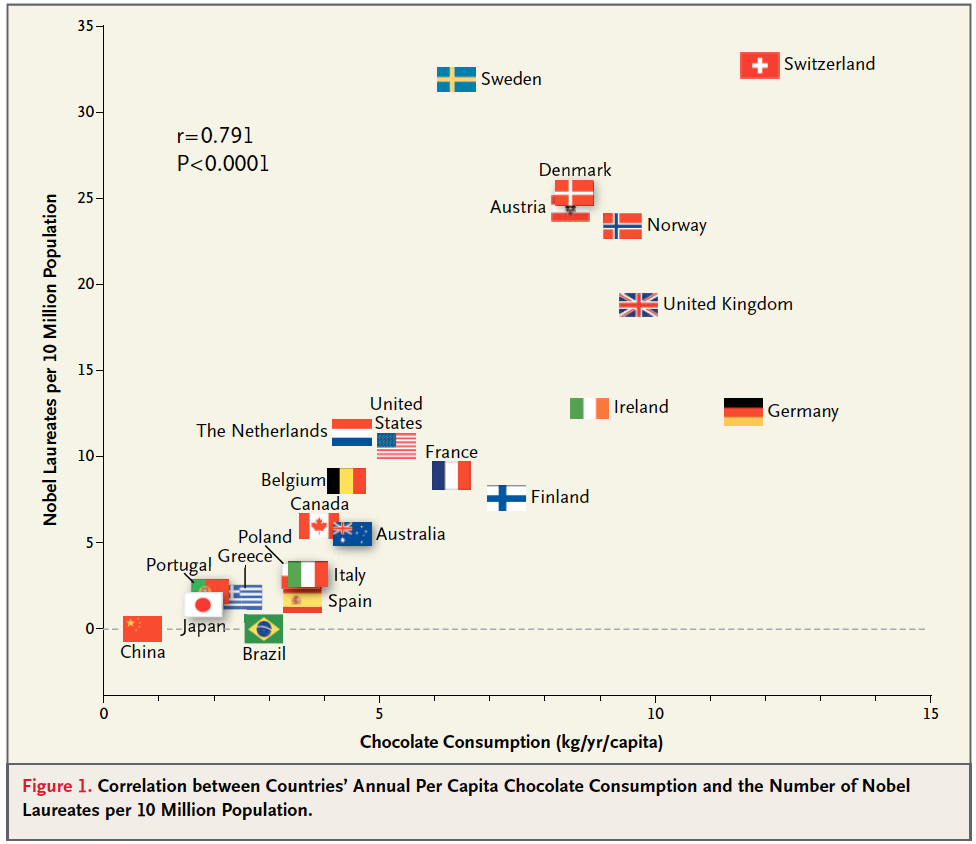
\includegraphics[width=0.8\textwidth]{chocolate_nobel.png}
  \centering
\includegraphics[width=0.8\textwidth]{messerli.pdf}

  \bigskip
  \tiny\begin{tabular}{ll}
    $N$: & Nobel Laureates (per $10^7$ capita);\\
    $C$: & Annual chocolate consumption (in kg/capita).
  \end{tabular}
\end{frame}

\begin{comment}
\begin{frame}{Hypothesis 1: $N$ causes $C$}
  ``Nobel prizes are celebrated with massive chocolate feasts''\\

  $\Sin = \{N\}$, $\Send = \{C\}$, $\Srnd = \emptyset$, $\theta = (\alpha,\beta) \in \RN^2$, $\C{X}_N = \RN$, $\C{X}_C = \RN$, $f_{\alpha,\beta} : (x_N,x_C) \mapsto \alpha + \beta x_N$.

  Structural equations:
    $$X_C^{\doit(x_N)} = \alpha + \beta x_N.$$
  
  For a given parameter $(\alpha,\beta)$, the iSCM has a unique solution function 
  $$g_{\alpha,\beta} : x_N \mapsto \alpha + \beta x_N,$$
  unique potential outcomes of the form 
  $$X_C^{\doit(x_N)} = \alpha + \beta x_N,$$
  and any conditional random variable $X : \C{U} \times \CXJ \to \CX$ that satisfies
  $$X_C = \alpha + \beta X_N$$
  is a solution of the iSCM.
\end{frame}
\end{comment}

\begin{frame}{Hypothesis 1: $C$ causes $N$}
  ``Chocolate contains brain enhancing chemicals''\\
   
  $\Sin = \{C\}$, $\Send = \{N\}$, $\Srnd = \emptyset$, $\theta = (\gamma,\delta) \in \CX_\Theta := \RN^2$, $\C{X}_C = \RN$, $\C{X}_N = \RN$, $f^{\gamma,\delta} : (x_C,x_N) \mapsto \gamma + \delta x_C$.

  Structural equations:
    $$X_N^{\doit(x_C)} = \gamma + \delta x_C.$$
  For a given parameter $\theta$, the iSCM $M^\theta$ has a unique solution function
    $$g^{\gamma,\delta} : x_C \mapsto \gamma + \delta x_C,$$
  unique potential outcomes of the form 
    $$X_N^{\doit(x_C)} = \gamma + \delta x_C,$$
  and any conditional random variable $X : \C{U} \times \CXJ \to \CX$ that satisfies
  $$X_C = \alpha + \beta X_N$$
  is a solution of the iSCM $M^\theta$.
\end{frame}

\begin{frame}{Hypothesis 2: $W$ causes $N$ and $C$}
  ``Inhabitants of wealthy countries eat more chocolate and conduct more scientific research''\\

  $\Sin = \emptyset$, $\Send = \{C,N\}$, $\Srnd = \{W\}$, $\theta = (\alpha,\beta,\gamma,\delta,\sigma) \in \RN^4 \times [0,\infty)$, $\C{X}_W = \RN$, $\C{X}_C = \RN$, $\C{X}_N = \RN$, $f^{\theta} : (x_C,x_N,x_W) \mapsto (\alpha + \beta x_W, \gamma + \delta x_W) \in \C{X}_C \times \C{X}_N$, $P^{\theta} = \C{N}(0,\sigma^2)$.

  Structural equations:
    \begin{align*}
      X_C & = \alpha + \beta X_W, \\
      X_N & = \gamma + \delta X_W.
    \end{align*}
  
  For a given parameter $\theta$, the SCM $M^{\theta}$ has unique solution function 
  $$g^\theta : x_W \mapsto (\alpha + \beta x_W, \gamma + \delta x_W) \in \C{X}_C \times \C{X}_N$$
  and outcomes of the form
  $$(X_C,X_N) = (\alpha + \beta X_W, \gamma + \delta X_W)$$ 
  for any random variable $X_W \sim \C{N}(0,\sigma^2)$.
\end{frame}

\begin{frame}{Samplers / data-generating processes}
  \begin{enumerate}
    \item[H1] $C$ causes $N$:\\
      \begin{algorithmic}[1]
        \Input $\gamma,\delta,n$
        \For{$i=1,\dots,n$}
          \Input $x_C^{(i)}$;
          \State $X_N^{(i)} \leftarrow \gamma + \delta x_C^{(i)}$;
          \Output $(x_C^{(i)},X_N^{(i)})$
        \EndFor
      \end{algorithmic}
    \item[H2] $W$ causes $C$ and $N$:\\
      \begin{algorithmic}[1]
        \Input $\alpha,\beta,\gamma,\delta,\sigma^2,n$
        \For{$i=1,\dots,n$}
          \Sample $X_W^{(i)} \sim \C{N}(0,\sigma^2)$;
          \State $X_C^{(i)} \leftarrow \alpha + \beta x_W^{(i)}$;
          \State $X_N^{(i)} \leftarrow \gamma + \delta x_W^{(i)}$.
          \Output $(X_C^{(i)},X_N^{(i)},X_W^{(i)})$
        \EndFor
      \end{algorithmic}
  \end{enumerate}
\end{frame}

\begin{frame}{Hard interventions}
  \begin{Def}[\ref{def:scm_hard_intervention}, \ref{def:scm_hard_intervention_stochastic}, \ref{def:scm_hard_intervention_unspecified}]
  Let $M = \lt \Sin, \Send, \Srnd, \CX, P, f \rt$ be an iSCM and $T \subseteq J \cup V$ the \emph{intervention target}. 
  We define three variants of \emph{hard interventions}:
    \begin{enumerate}
      \item For a \emph{specified target value} $\xi_T \in \CX_T$, define
    $$M_{\doit(X_T=\xi_t)} = \lt J\setminus T, V \cup T, W, \CX, P, (f_{V\setminus T},\xi_T)\rt$$
  \item For a \emph{stochastic target value} with distribution $Q_T \in \bigotimes_{t\in T} \C{P}(\CX_t)$, define
    $$M_{\doit(X_T\sim Q_T)} = \lt J\setminus T, V \setminus T, W \cup T, \CX, P \otimes Q_T, f_{V\setminus T}\rt$$
  \item For an \emph{unspecified target value}, define
    $$M_{\doit(T)} = \lt J\cup T, V\setminus T, W, \CX, P, f_{V\setminus T} \rt$$
    \end{enumerate}
  \end{Def}
\end{frame}

\begin{frame}{Soft interventions (mechanism changes)}
%Soft interventions replace the causal mechanism of an endogenous variable by another causal mechanism,
%or the exogenous distribution of an exogenous random variable by another distribution.
\begin{Def}[\ref{def:scm_soft_intervention}]
  Given an iSCM $M = \lt \Sin, \Send, \Srnd, \CX, P, f \rt$, an intervention target $T \subseteq \Send$, 
  and measurable functions $\tilde{f}_v : \CX \to \CX_v$ for $v \in T$,
  a \emph{soft intervention on $M$ replacing $f_T$ by $\tilde f_T$} yields an intervened iSCM of the form
  %$$\tilde{M} := \lt \Sin,\Send,\Srnd,\CX,\tilde{P},\tilde{f} \rt$$
  $$M_{\doit(T \ot \tilde{f}_T)} := \lt \Sin,\Send,\Srnd,\CX,P,(f_{V\sm T}, \tilde{f}_T) \rt.$$
\end{Def}
\end{frame}

\begin{frame}{Intervention variables---Example}
  \emph{Intervention variables} encode whether/how an intervention is performed.
  \begin{example}
    Consider an SCM with endogenous variables $X_1,X_2$, exogenous random variables $E_1,E_2$ and structural equations:
    $$X_1 = f_1(X_2,E_1), \qquad
      X_2 = f_2(X_1,E_2) \phantom{x_2}$$
    After a hard intervention $\doit(X_2=x_2)$ the structural equations become:
    $$X_1 = f_1(X_2,E_1), \qquad
      X_2 = x_2 \phantom{f_2(X_1,E_2)}$$
    We can combine both into a single iSCM by adding an intervention variable $I_2$ (an exogenous input variable) and change the structural equations into:
    $$X_1 = f_1(X_2,E_1), \qquad
      X_2 = \begin{cases}
        f_2(X_1,E_2) & I_2 = 0 \\
        x_2          & I_2 = 1
      \end{cases}$$
  \end{example}
\end{frame}

\begin{frame}{Intervention variables---Special case}
  \begin{Def}[\ref{def:scm_intervention_variables}]
  Let $M = \lt \Sin, \Send, \Srnd, \CX, P, f \rt$ be an iSCM, and $B \subseteq V \cup J$.
  For each $b \in B \cap V$, we introduce an additional `intervention variable' $I_b$ as exogenous input variable; for $j \in B \cap J$, we just set $I_j := j$.
  We denote $I_B := (I_b)_{b \in B}$.
  We define an extended iSCM 
  \vskip-2mm
  $$\textstyle M_{\doit(I_B)} := \lt \Sin \cup I_B, \Send, \Srnd, \CX \times \prod_{b \in B \cap V} \CX_{I_b}, P, \tilde{f} \rt$$
  with $\CX_{I_b} := \CX_b \,\dot\cup\, \{\star\}$, with causal mechanism $\tilde{f}$ with components
  \vskip-6mm
  \begin{align*}
    v \in V \cap B: \qquad &\tilde{f}_v(x_{V \cup J \cup W \cup I_B}) := \begin{cases}
      f_v(x_{V \cup J \cup W}) & x_{I_v} = \star \\
      x_{I_v} & x_{I_v} \in \CX_v
    \end{cases}\\
    v \in V \sm B: \qquad & \tilde{f}_v(x_{V \cup J \cup W \cup I_B}) := f_v(x_{V \cup J \cup W})
  \end{align*}
  \vskip-2mm
  For $b \in B \cap V$, $x_{I_b} = \star$ encodes that there is no intervention on $b$, while $x_{I_b} \ne \star$ encodes that the hard intervention $\doit(X_b = x_{I_b})$ is performed.
\end{Def}
Purpose: jointly encode $\{M_{\doit(X_C)} : C \subseteq B\}$ into a single iSCM $M_{\doit(I_B)}$.
\end{frame}

\begin{frame}{Interventions with disjoint targets commute}
\begin{Prp}[\ref{prp:interventions_commute}, \ref{prp:adding_intervention_variables_one_by_one}, \ref{prp:adding_intervention_variables_commutes}]
Let $M = \lt \Sin, \Send, \Srnd, \CX, P, f \rt$ be an iSCM.
  \begin{itemize}
    \item
(Hard or soft) interventions $\doit(T_1\dots)$, $\doit(T_2\dots)$ with disjoint targets $T_1, T_2 \subseteq \Sin \cup \Send$ (of any of the four variants) commute:
  $$(M_{\doit(T_1\dots)})_{\doit(T_2\dots)} = (M_{\doit(T_2\dots)})_{\doit(T_1\dots)}.$$
\item
Adding intervention variable $b_1 \ins V \cup J$ and $b_2 \ins V \cup J$ (with $b_1 \ne b_2$) commutes:
  $$(M_{\doit(I_{b_1})})_{\doit(I_{b_2})} = (M_{\doit(I_{b_2})})_{\doit(I_{b_1})} = M_{\doit(I_{\{b_1,b_2\}})}.$$
\item 
  Adding intervention variables to $B \subseteq V \cup J$ commutes with (hard or soft) interventions $\doit(T\dots)$ with disjoint target $T \subseteq \Sin \cup \Send$ (of any of the four variants):
  $$(M_{\doit(I_B)})_{\doit(T\dots)} = (M_{\doit(T\dots)})_{\doit(I_B)}.$$
  \end{itemize}
\end{Prp}
\end{frame}

\begin{frame}{Decomposition}
  If we think about an iSCM as modeling a ``system'', then we also obtain a model for a ``subsystem'' in the following way.

  \begin{Def}[\ref{def:sub_scm}]
  Given an iSCM $M = \lt \Sin, \Send, \Srnd, \CX, P, f \rt$ and a subset $V' \subseteq V$ of its endogenous variables, we define its \emph{submodel on $V'$} as the iSCM
    $$M^{[V']} := \lt \Sin \cup (V \sm V'), V', W,\CX,P,f_{V'} \rt.$$
  \end{Def}
  Note that this is just the intervened iSCM $M^{\doit(V \sm V')}$.
\end{frame}

\begin{frame}{Composition, Modularity}
%Given two SCMs, such that some of the variables of one SCM can be used as (part of the) exogenous input of the other, and possibly vice versa, we can compose them into a single SCM.
  \begin{itemize}
    \item Definition~\ref{def:compose_scm}: a \emph{composition} operation that ``connects'' some of the inputs of one iSCM to the outputs of another, and vice versa.
    \item Decomposition (taking submodels) is `dual to' composition (combining submodels).
    \item These operations formalize the notion of \emph{modularity}: an iSCM models a system of interacting components.
    \item `Atomic' submodels consisting of a single endogenous variable cannot be further decomposed.
  \end{itemize}      
\end{frame}

\begin{frame}{Essentially unique (partial) solvability}
\begin{Def}[\ref{def:scm_unique_solvability}]
  Let $M = \lt \Sin, \Send, \Srnd, \CX, P, f \rt$ be an iSCM.
  \begin{itemize}
    \item
  We say that $M$ is \emph{essentially uniquely solvable} if there exists a measurable function $g : \CX_J \times \CX_W \to \CX_V$ that satisfies
    $$x_V = f(x) \iff x_V = g(x_J,x_W)\quad M\as.$$
  \item
  For a subset $L \ins V$, we say that $M$ is \emph{essentially uniquely solvable w.r.t.\ $L$} if there exists a measurable function $g^{[L]} : \CX_J \times \CX_{(V\sm L)} \times \CX_W \to \CX_L$ that satisfies
    $$x_L = f_L(x) \iff x_L = g^{[L]}(x_J,x_{(V\sm L)},x_W)\quad M\as.$$
  \end{itemize}
\end{Def}
Note that such a function $g$ is a solution function of $M$, and $g^{[L]}$ is a partial solution function of $M$ w.r.t.\ $L$.
Hence, if $M$ is essentially uniquely solvable (w.r.t.\ $L$), then $M$ is solvable (w.r.t.\ $L$).
\end{frame}

\begin{frame}{Essential uniqueness of (partial) solution functions}
\begin{Def}[\ref{def:scm_essentially_unique_solution_function}]
  Let $M = \lt \Sin, \Send, \Srnd, \CX, P, f \rt$ be an iSCM.
  \begin{itemize}
    \item
  We say that its solution function is \emph{essentially unique} if $g = \tilde{g}\ M\as$ for any two solution functions $g,\tilde{g}$ of $M$.
\item
  We say that its partial solution function w.r.t.\ $L \ins V$ is \emph{essentially unique} if $g^{[L]} = \tilde{g}^{[L]}\ M\as$ for any two partial solution functions $g^{[L]}, \tilde{g}^{[L]}$ of $M$ w.r.t.\ $L$.
  \end{itemize}
\end{Def}
A simple (but useful) consequence:
\begin{Prp}[\ref{prp:scm_essentially_unique_solution_functions}]
  Suppose that iSCM $M$ is essentially uniquely solvable w.r.t.\ $L \ins V$.
  Then for any partial solution function $\tilde{g}^{[L]}$ of $M$ w.r.t.\ $L$ we have:
    $$x_L = f_L(x) \iff x_L = \tilde{g}^{[L]}(x_J,x_{(V\sm L)},x_W)\quad M\as.$$
  Hence, the partial solution function of $M$ w.r.t.\ $L$ is essentially unique.
\end{Prp}
\end{frame}

\begin{frame}{Essentially Unique Solvability---Properties}
\begin{Thm}[\ref{thm:scm_essentially_unique_solvability_implies}]
  Let $M = \lt \Sin, \Send, \Srnd, \CX, P, f \rt$ be an iSCM.
  If $M$ is essentially uniquely solvable, then its solution function is essentially unique, and:
  \begin{enumerate}
    \item The distribution of a potential outcome $X^{\doit(\xJ)}_{V\cup W}$ for input $\xJ\in\XJ$ is unique and given by 
      $$X_{V\cup W}^{\doit(\xJ)} \sim (g^{\doit(\xJ)},\id_{\CXW})_* P_M(X_W),$$
      where $g^{\doit(\xJ)} : \CXW \to \CXV : \xW \mapsto g(x_J,\xW)$ with $g : \CXJ \times \CXW \to \CXV$ a solution function of $M$.
    \item $M$ has a unique Markov kernel given by
      $$P_{M}(\XV,\XW \mid\doit(\XJ)) = (g,\id_{\CXW})_* \lp \bigg( \bigotimes_{w\in W} P_w(X_w) \bigg) \otimes \delta(X_J|X_J) \rp$$
      for $g : \CXJ \times \CXW \to \CXV$ a solution function of $M$.
  \end{enumerate}
\end{Thm}
\end{frame}

\begin{frame}{Example: Linear iSCMs}
\begin{Def}[\ref{def:linear_scms}]
Let $\mathbb{K}$ be a field.
Let $M=\lt \Sin, \Send, \Srnd, \CX, P, f \rt$ be an iSCM, where each $\CX_v$ is a finite-dimensional Polish vector space over $\mathbb{K}$.
Then $M$ is called \emph{essentially linear} if the causal mechanisms are affine in $X_V$:
$$
  f_v(x_J,x_W,x_V) = \sum_{u\in V} B_{uv}(x_J,x_W) x_u + c_v(x_J,x_W) \qquad M\as,
$$
where for all $x_J \in \CX_J$ and all $x_W \in \CX_W$, $B_{uv}(x_J,x_W) : \CX_u \to \CX_v$ is linear and $c_v(x_J,x_W) \in \CX_v$ for all $u,v \in V$.
\end{Def}
\begin{Prp}[\ref{prp:linear_scms}]
$M$ is essentially uniquely solvable if the matrices $I-B(x_J,x_W)$ are invertible for all $x_J \in \CX_J, x_W \in \CX_W$ up to a measurable $M$-null set.
The corresponding essentially unique solution function is:
\small $$g : \CX_J \times \CX_W \to \CX_V : (x_J,x_W) \mapsto (I - B(x_J,x_W))^{-1} \big(B(x_J,x_W) x_V + c(x_J,x_W)\big).$$
\end{Prp}
\end{frame}

\begin{frame}{Simple iSCMs}
After an intervention, an iSCM may no longer be essentially uniquely solvable.

For simplicity, we consider mostly `simple' iSCMs:
\begin{Def}[\ref{def:simple_scm}]
  An iSCM $M = \lt \Sin, \Send, \Srnd, \CX, P, f \rt$ is called \emph{simple} if for all $T \subseteq \Send$, $M$ is essentially uniquely solvable w.r.t.\ $T$.
\end{Def}
Note that this includes essentially unique solvability of $M$ itself for $T = \emptyset$.

Proposition~\ref{prp:scm_partial_solvability} gives:
\begin{Rem}
If for each $L \ins V$, 
$$[\exists! x_L \in \CX_L : x_L = f_L(x_J,x_{V\sm L},x_W,x_L)]$$
holds up to a measurable $M$-null set, then $M$ is a simple iSCM.
\end{Rem}
\end{frame}

\begin{frame}{Example of simple iSCM}
\begin{Eg}[\ref{eg:simple_scm}]
Consider an iSCM with structural equations
$$X_1 = W_1 \qquad X_2 = W_2 \qquad X_3 = X_1 X_4 + W_3 \qquad X_4 = X_2 X_3 + W_4 $$
where the $X$'s are considered endogenous real variables and the $W$'s exogenous variables with domains $(-1,1)$.
We can solve the system of structural equations with respect to $X$ in terms of $W$:
$$X_1 = W_1 \qquad X_2 = W_2 \qquad X_3 = \frac{W_3 + W_1 W_4}{1 - W_1 W_2} \qquad X_4 = \frac{W_2 W_3 + W_4}{1 - W_2 W_1}$$
Similarly, we can take any subset of the structural equations and solve it with respect to the variables appearing on the l.h.s.\ in terms of the variables appearing on the r.h.s.\ of the equations in the subset, and obtain a unique solution. Thus this iSCM is simple.
%For example, only solving the structural equations for $X_3$ and $X_4$, we obtain:
%$$X_3 = \frac{W_3 + W_1 W_4}{1 - W_1 X_2} \qquad X_4 = \frac{W_2 W_3 + W_4}{1 - W_2 X_1}$$
%where the variables $X_1$ and $X_2$ are now considered as exogenous input variables (instead of endogenous variables).
%Hence, any subset of the structural equations has a unique solution for the variables appearing on the l.h.s.\ in terms
%of the remaining ones on the r.h.s., which means that this SCM is simple.
\end{Eg}
We will see later that all acyclic iSCMs are simple.
\end{frame}

\begin{frame}{Simple iSCMs---Properties}
Simplicity is preserved by hard interventions and by adding intervention variables.
\begin{Prp}[\ref{prp:scm_simplicity_preserved_by_interventions}]
  Let $M = \lt \Sin, \Send, \Srnd, \CX, P, f \rt$ be a simple iSCM. Then:
    \begin{enumerate}
      \item $M_{\doit(T\dots)}$ is simple for $T \subseteq V \cup J$ (hard interventions of all three types);
      \item $M_{\doit(I_B)}$ is simple for $B \subseteq V \cup J$ (adding intervention variables).
    \end{enumerate}
\end{Prp}
\begin{Cor}[\ref{cor:simple_scm}]
  If an iSCM $M$ is simple, then its Markov kernel $P_{M}(X_V, X_W \mid \doit(X_J))$ and all intervened Markov kernels
  $$P_{M_{\doit(T)}}(X_{V \sm T},X_W \mid \doit(X_{J \cup T}))$$
  for $T \subseteq V$ % \cup W$ 
  exist and are unique.
\end{Cor}
\end{frame}

\begin{frame}{Terminology}
\begin{Not}[\ref{not:scm_do_operator}]
  For a simple iSCM $M$, we write for $T \subseteq V$:
  $$P_{M}(X_{V \sm T}, X_W \mid \doit(X_J),\doit(X_T)) := P_{M_{\doit(T)}}(X_{V \sm T},X_W \mid \doit(X_{J \cup T}))$$
  We establish the following terminology for these Markov kernels:

  \medskip
  \centerline{\begin{tabular}{ll}
    Markov kernel & name \\
    \hline
    $P_M(X_{V\sm T} \mid \doit(X_J),\doit(X_T))$ & \emph{interventional Markov kernels of $M$} \\
    $P_M(X_V \mid \doit(X_J))$ & \emph{observable Markov kernel of $M$} \\
    $P_M(X_V)$ & \emph{observational Markov kernel of $M$}
  \end{tabular}}
\end{Not}
\end{frame}

\begin{frame}{Relations between causal models}
  \centerline{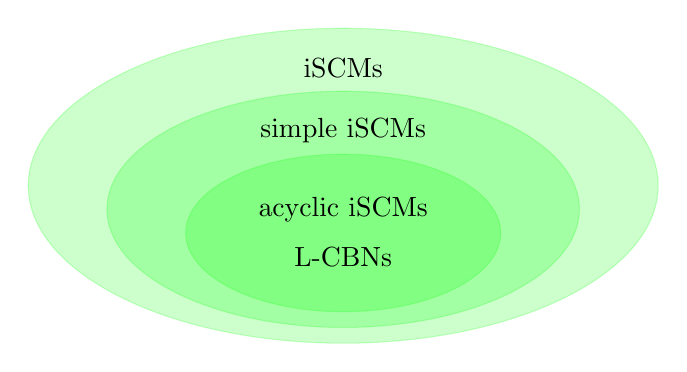
\begin{tikzpicture}
      \begin{scope}
%        \draw[draw=green,fill=green,opacity=0.2] (0,0) ellipse (1.5cm and 0.5cm);
        \draw[draw=green,fill=green,opacity=0.2] (0,0.3) ellipse (2cm and 1cm);
        \draw[draw=green,fill=green,opacity=0.2] (0,0.6) ellipse (3cm and 1.5cm);
        \draw[draw=green,fill=green,opacity=0.2] (0,0.9) ellipse (4cm and 2cm);
%        \draw[draw=green,fill=green,opacity=0.2] (0,1.2) ellipse (5cm and 2.5cm);
        \node at (0,0) {L-CBNs};
        \node at (0,0.6) {acyclic iSCMs};
        \node at (0,1.6) {simple iSCMs};
        \node at (0,2.4) {iSCMs};
%        \node at (0,3.2) {BCMs};
      \end{scope}
  \end{tikzpicture}}

  \bigskip
  \begin{itemize}
    \item L-CBNs are ``equivalent'' to acyclic iSCMs (Section~\ref{sec:acyclic_scms}).
    \item Simple iSCMs are more expressive than L-CBNs, because they can model (sufficiently weak) causal cycles.
    \item The class of iSCMs can deal with stronger feedback at the cost of much complexity.
  \end{itemize}
\end{frame}

